\documentclass{beamer}

\usetheme{Madrid}
\usecolortheme{beaver}

\title{Interaktivna igra Pong}
\subtitle{Projektna naloga pri predmetu Interaktivnost in oblikovanje informacij}
\author{Justin Raišp}
\date{14.1.2025}

\begin{document}

\begin{frame}
    \titlepage
\end{frame}

\begin{frame}{Pregled projekta}
    \textbf{Interaktivna igra Pong} je posodobljena različica klasične igre Pong, zasnovana za zabavno in prilagodljivo igralno izkušnjo. Igralci lahko uživajo v:
    \begin{itemize}
        \item nastavljivi hitrosti žogice za različne intenzivnosti igre,
        \item posebnih sposobnostih, kot so hitrejši udarci ali nevidne žogice,
        \item prilagoditvi ciljnega rezultata (npr. 3, 5, 7 ali 11 točk),
        \item dinamičnih ovirah, ki spreminjajo smer žogice.
    \end{itemize}
    \textbf{Glavna lastnost igre je, da se jo igra s pomočjo video kamere, ki sledi igralčevim rokam. Igralec premika svoj lopar s kazalcem.}
\end{frame}

\begin{frame}{Slike projekta}
  \begin{figure}
      \centering
      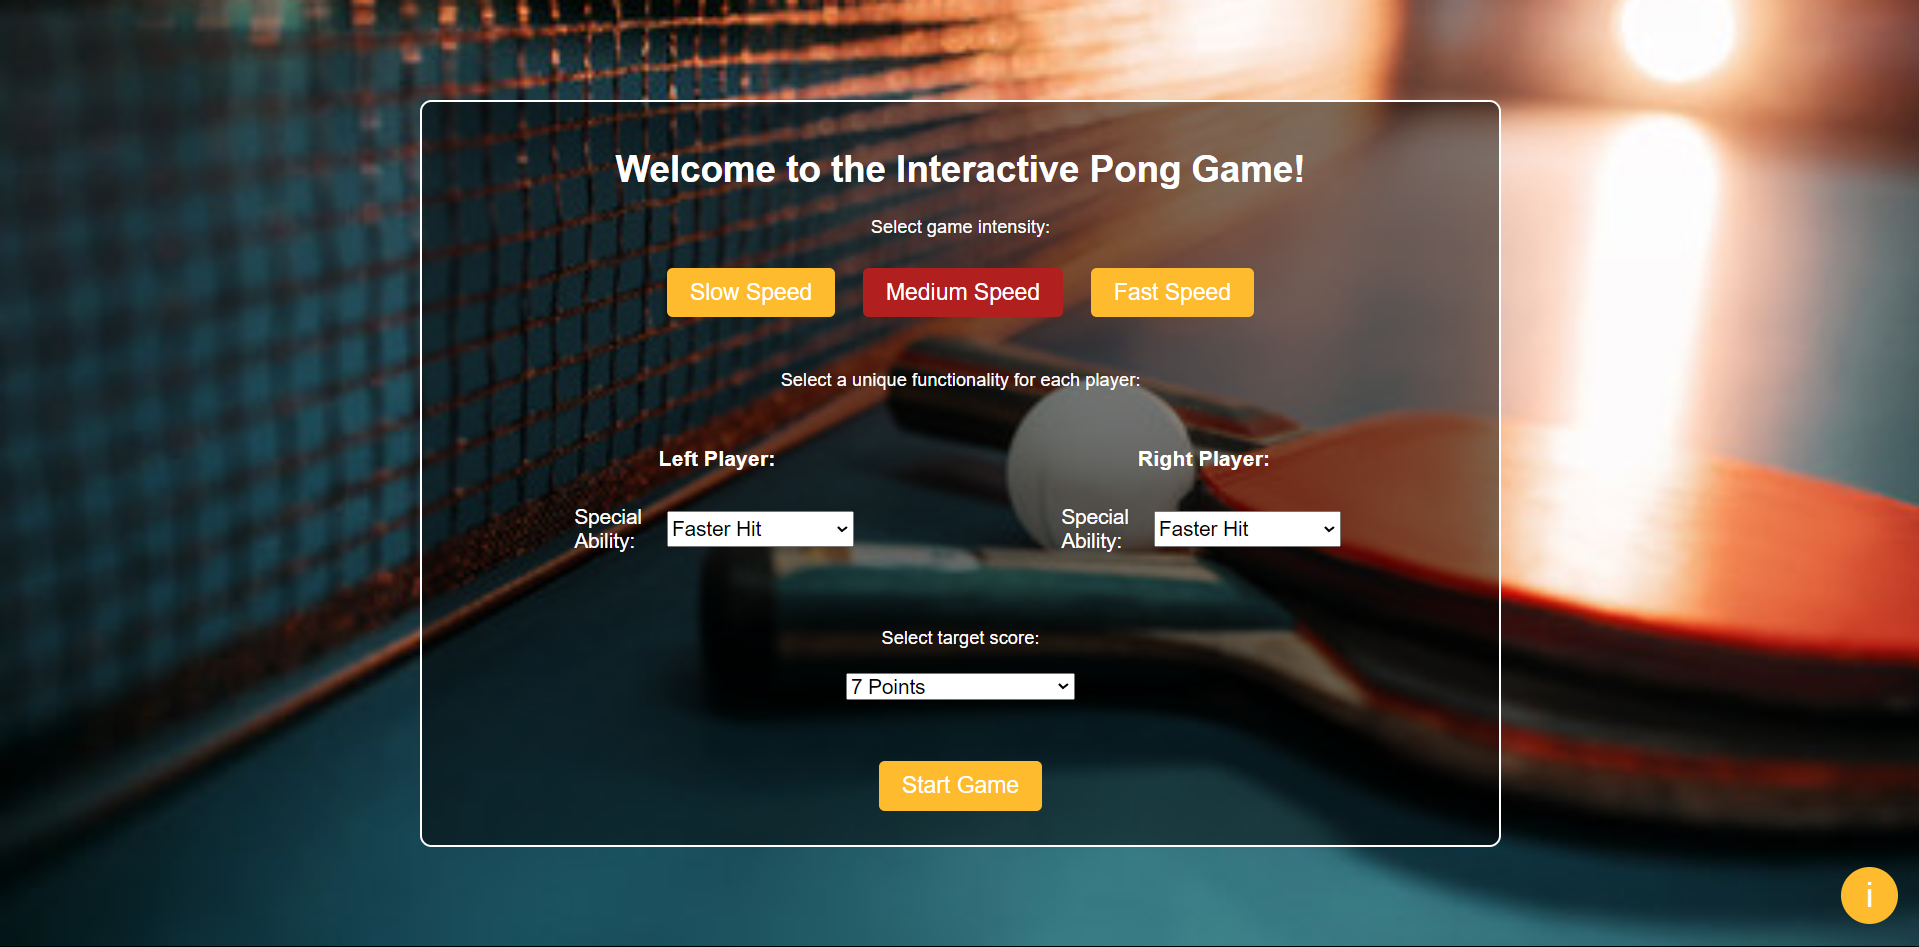
\includegraphics[width=0.9\textwidth]{images/homePage.png}
      \caption{Začetna stran.}
      \label{fig:interface}
  \end{figure}
\end{frame}

\begin{frame}{Slike projekta}
  \begin{figure}
      \centering
      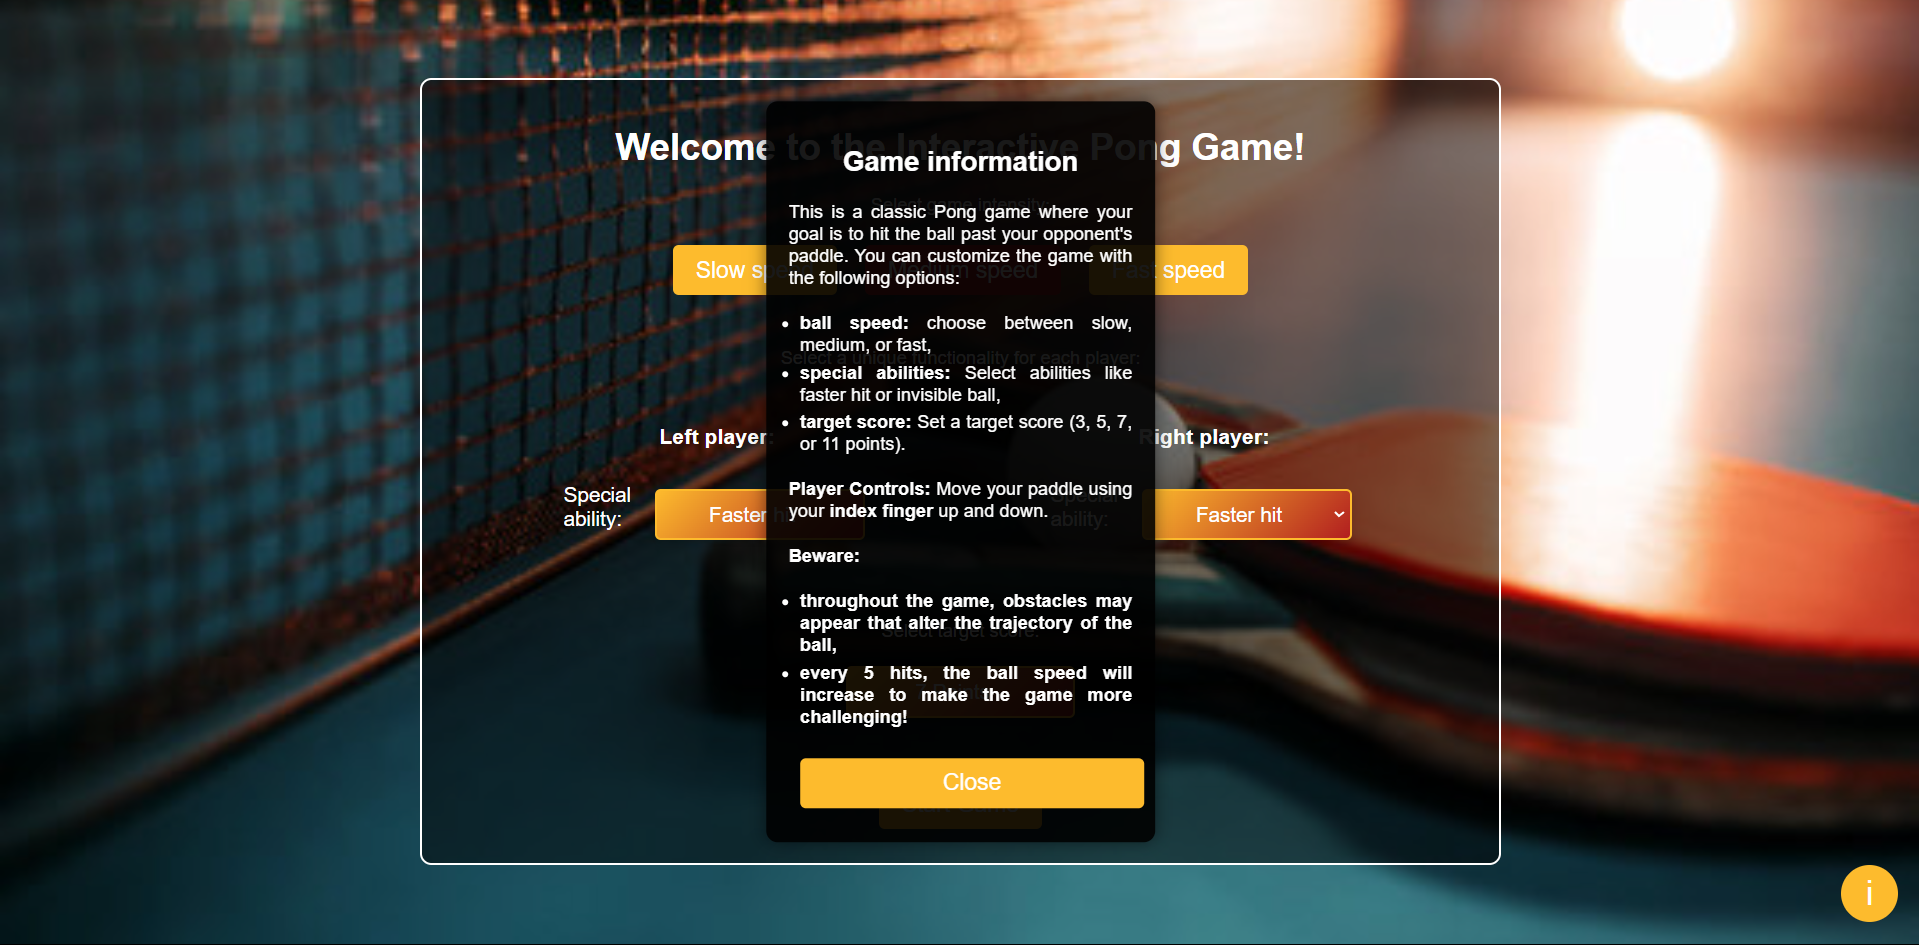
\includegraphics[width=0.9\textwidth]{images/info.png}
      \caption{Informacije.}
      \label{fig:interface}
  \end{figure}
\end{frame}

\begin{frame}{Slike projekta}
  \begin{figure}
      \centering
      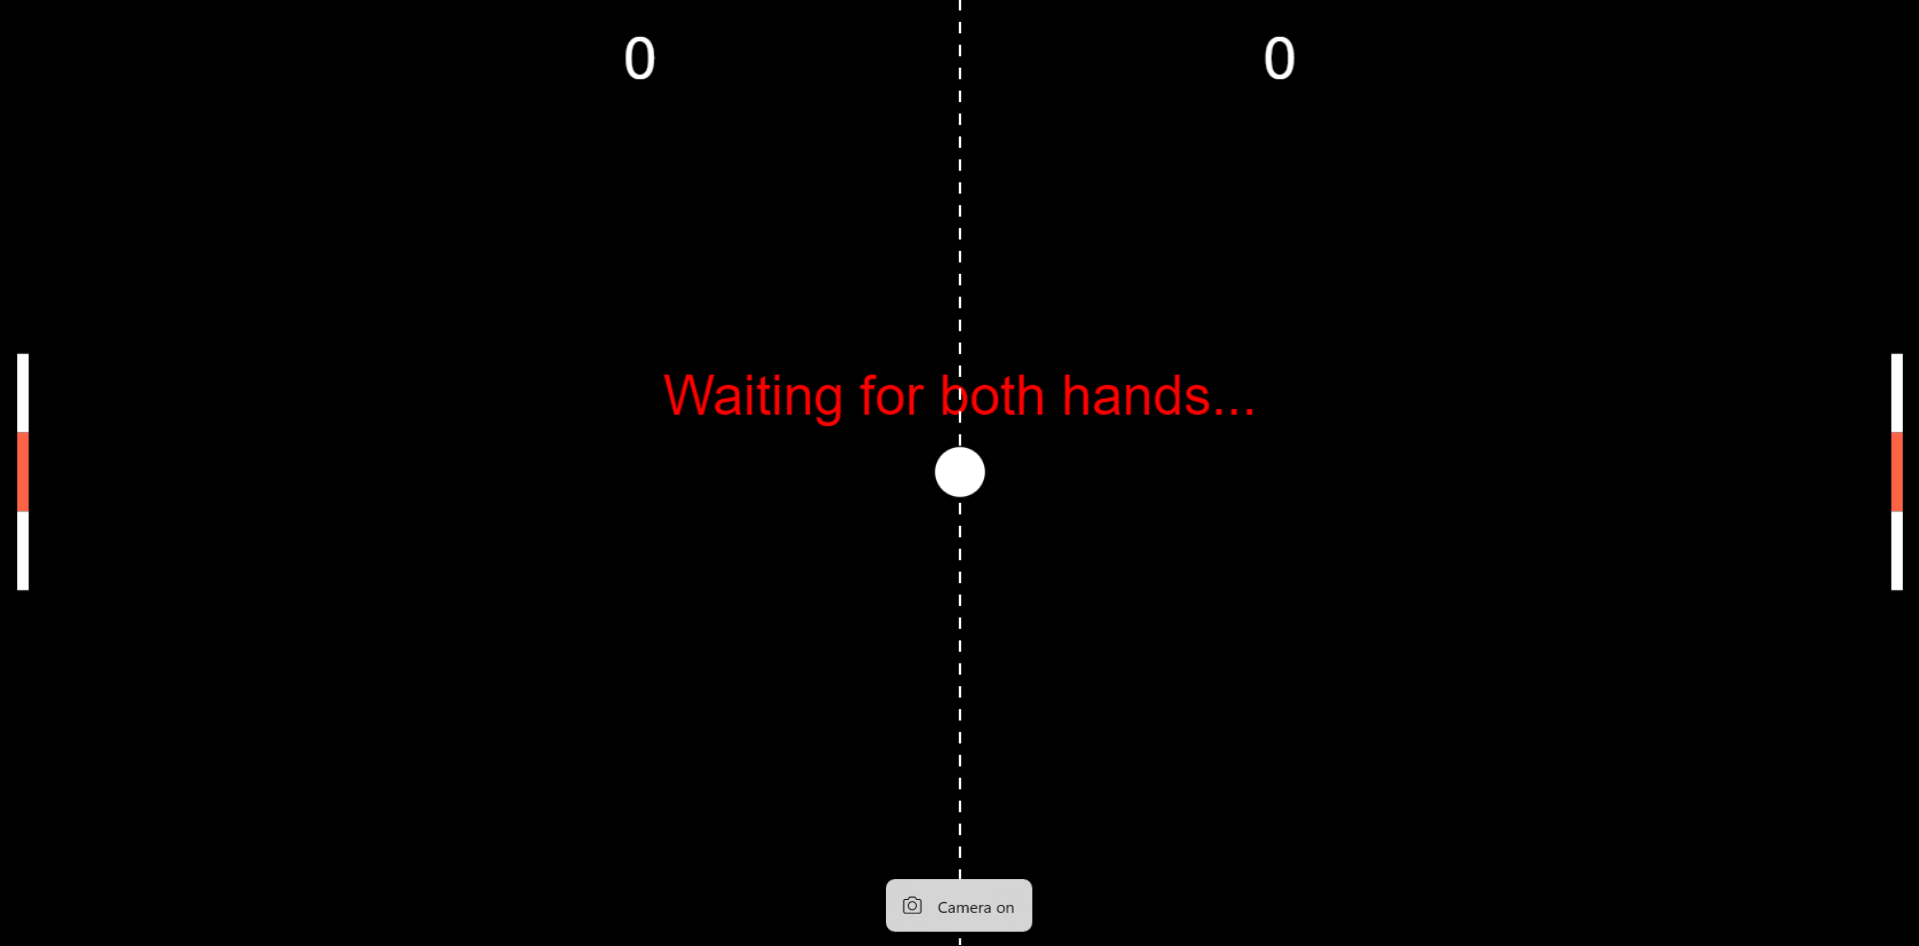
\includegraphics[width=0.9\textwidth]{images/startOfGame.png}
      \caption{Delovanje igre z uporabo kamere.}
      \label{fig:camera}
  \end{figure}
\end{frame}


\begin{frame}{Slike projekta}
  \begin{figure}
      \centering
      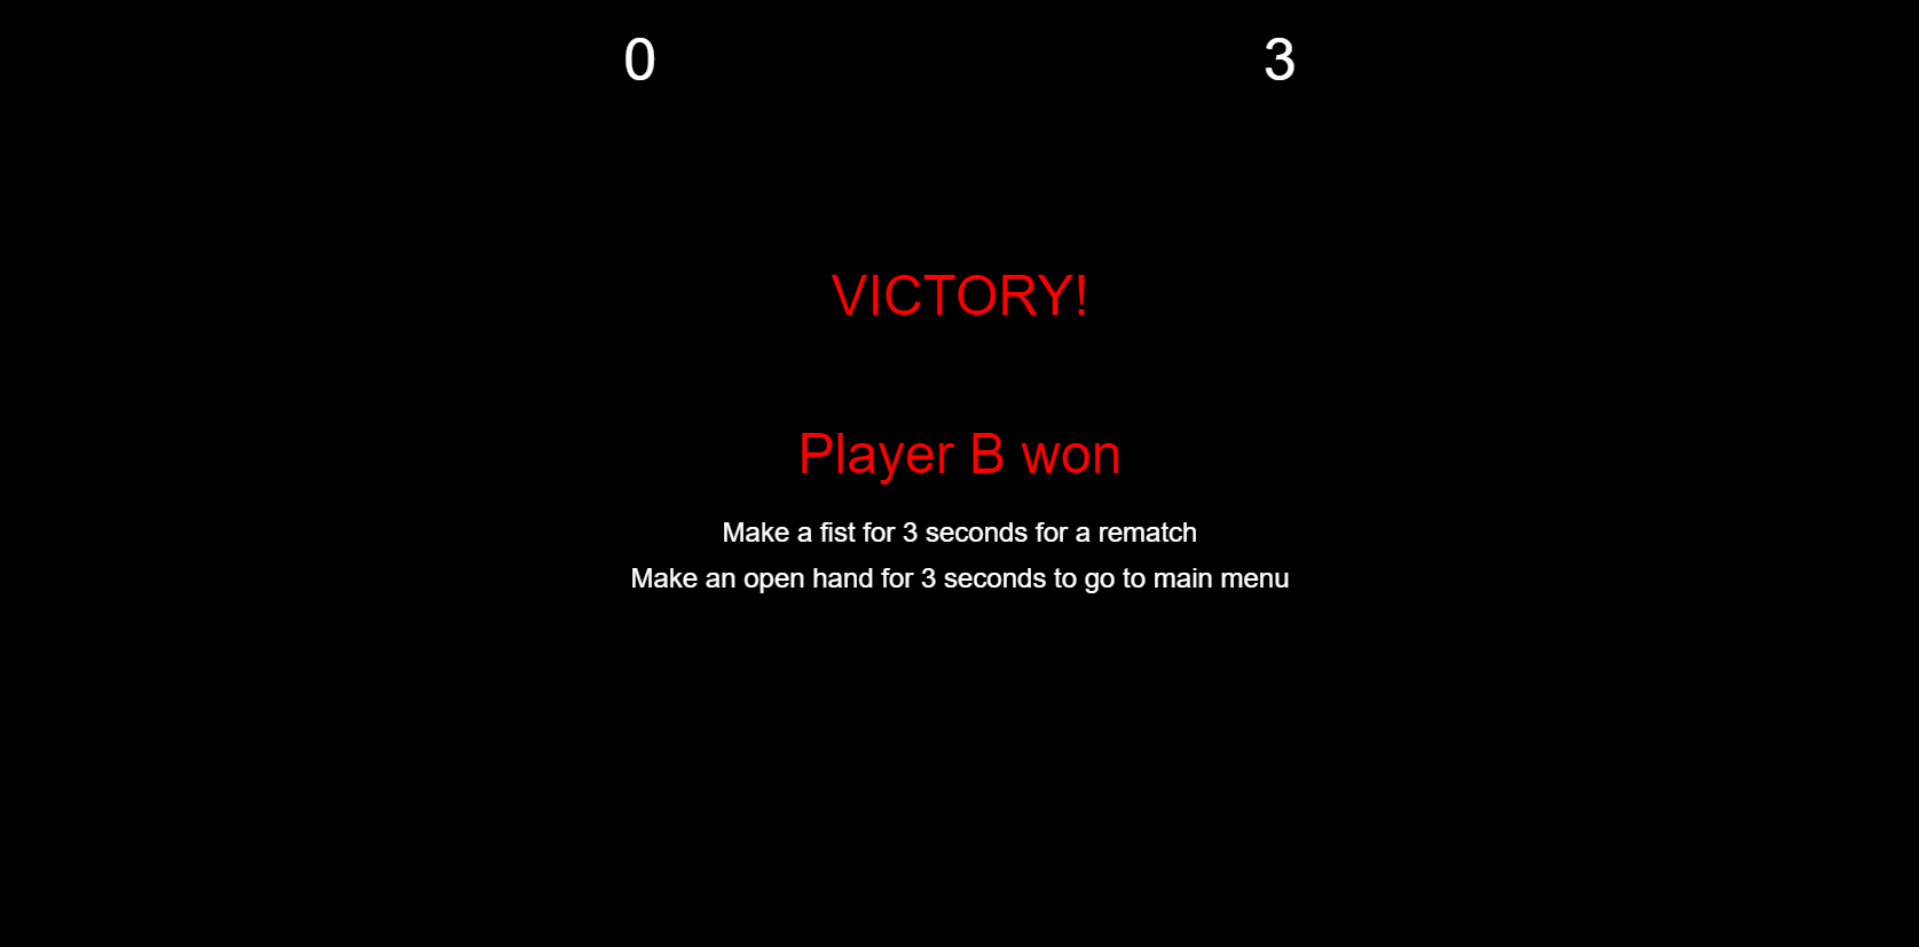
\includegraphics[width=0.9\textwidth]{images/endOfGame.png}
      \caption{Zaključek igre.}
      \label{fig:camera}
  \end{figure}
\end{frame}

\begin{frame}{Cilji projekta}
    Glavni cilji, zastavljeni za ta projekt, so bili:
    \begin{enumerate}
        \item razviti interaktivno različico klasične igre Pong, kjer se z rokami upravlja z loparji,
        \item implementirati možnosti prilagodljive igre, vključno z:
            \begin{itemize}
                \item nastavljivo hitrostjo žogice,
                \item posebnimi sposobnostmi za vsakega igralca,
                \item konfiguracijo ciljnega rezultata.
            \end{itemize}
        \item vpeljati zvočne učinke za izboljšanje uporabniške izkušnje,
        \item uvesti dinamične ovire za povečanje zahtevnosti igre,
        \item zagotoviti, da je igra odzivna in deluje na različnih velikostih zaslonov,
        \item gostiti igro na spletu za lahek dostop na:
        \begin{center}
            \textbf{\url{https://justinraisp.github.io/Interactive-pong-game/}}
        \end{center}
    \end{enumerate}
\end{frame}

\begin{frame}{Zaključek}
    Ta projekt združuje nostalgično zabavo igre Pong s sodobnimi igralnimi funkcijami, da ponudi privlačno in zahtevno izkušnjo. Možnosti prilagajanja in dostopnost prek spleta zagotavljajo, da je igra privlačna za širok spekter uporabnikov. \\
    
    \bigskip
    \textbf{Več informacij na spletni strani repozitorija:} \\
    \url{https://github.com/justinraisp/Interactive-pong-game}
\end{frame}

\end{document}
